\documentclass[border=3pt,tikz]{standalone}
\usepackage[T1]{fontenc}
\usepackage[scaled]{helvet}
\renewcommand{\familydefault}{\sfdefault}
\usepackage{amsmath}
\usetikzlibrary{arrows.meta,positioning,calc,fit,backgrounds}

\definecolor{sensorfill}{RGB}{157,195,230}
\definecolor{sensordraw}{RGB}{46,117,182}
\definecolor{yellfill}{RGB}{255,242,204}
\definecolor{yelldraw}{RGB}{197,110,20}
\definecolor{wavecol}{RGB}{197,110,20}
\definecolor{greenfill}{RGB}{198,224,180}
\definecolor{redfill}{RGB}{247,196,193}
\definecolor{kalfill}{RGB}{222,235,247}
\definecolor{kaldraw}{RGB}{47,84,150}
\definecolor{dashblue}{RGB}{0,112,192}

\begin{document}
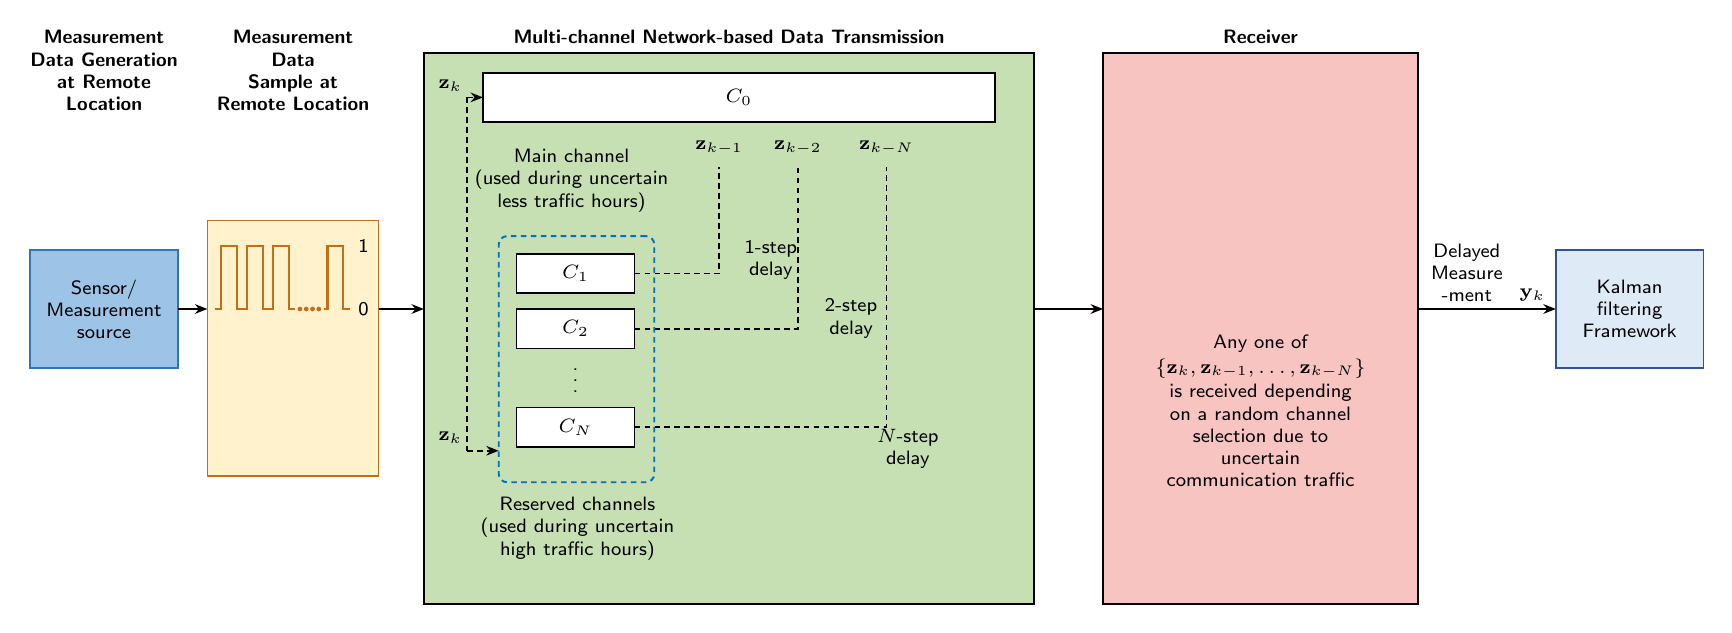
\begin{tikzpicture}[
  font=\sffamily\scriptsize,
  >={Stealth[length=4.5pt,width=3.5pt]},
  blk/.style={draw=black,line width=0.6pt,align=center,inner sep=1pt},
  lbl/.style={align=center,inner sep=1pt},
  ttl/.style={align=center,inner sep=1pt,font=\sffamily\scriptsize\bfseries},
  flow/.style={->,line width=0.7pt},
  dsh/.style={dashed,dash pattern=on 2pt off 1.6pt,line width=0.6pt},
]

%======================= BACKGROUND PANELS =======================
% Green panel : multi-channel network
\node[blk,fill=greenfill,minimum width=7.75cm,minimum height=7cm] (green) at (9.25,3.75) {};
% Red panel : receiver
\node[blk,fill=redfill,minimum width=4cm,minimum height=7cm] (red) at (16.00,3.75) {};

%======================= COLUMN TITLES =======================
\node[ttl,anchor=north] at (1.3125,7.58)
  {Measurement\\Data Generation\\at Remote\\Location};
\node[ttl,anchor=north] at (3.7125,7.58)
  {Measurement\\Data\\Sample at\\Remote Location};
\node[ttl,anchor=north] at (9.25,7.58) {Multi-channel Network-based Data Transmission};
\node[ttl,anchor=north] at (16.00,7.58) {Receiver};

%======================= BLOCK 1 : SENSOR =======================
\node[blk,fill=sensorfill,draw=sensordraw,minimum width=1.875cm,minimum height=1.5cm]
  (sensor) at (1.3125,4.00) {Sensor/\\Measurement\\source};

%======================= BLOCK 2 : DATA SAMPLE =======================
\node[blk,fill=yellfill,draw=yelldraw,minimum width=2.175cm,minimum height=3.25cm]
  (samp) at (3.7125,3.50) {};
% square wave
\draw[wavecol,line width=0.9pt]
  (2.72,4.00) -- (2.80,4.00) -- (2.80,4.80) -- (3.00,4.80) -- (3.00,4.00)
  -- (3.13,4.00) -- (3.13,4.80) -- (3.33,4.80) -- (3.33,4.00)
  -- (3.46,4.00) -- (3.46,4.80) -- (3.66,4.80) -- (3.66,4.00) -- (3.74,4.00);
\foreach \x in {3.80,3.88,3.96,4.04}{\fill[wavecol] (\x,4.00) circle (0.030);}
\draw[wavecol,line width=0.9pt]
  (4.10,4.00) -- (4.15,4.00) -- (4.15,4.80) -- (4.35,4.80) -- (4.35,4.00) -- (4.44,4.00);
\node[lbl,anchor=west] at (4.50,4.80) {1};
\node[lbl,anchor=west] at (4.50,4.00) {0};

%======================= GREEN PANEL CONTENTS =======================
% main channel C0
\node[blk,fill=white,minimum width=6.5cm,minimum height=0.625cm] (c0) at (9.375,6.6875) {$C_0$};
\node[lbl] at (7.25,5.63) {Main channel\\(used during uncertain\\less traffic hours)};

% reserved channels group
\node[draw=dashblue,dsh,line width=0.7pt,rounded corners=3pt,
      minimum width=1.975cm,minimum height=3.125cm] (grp) at (7.3125,3.3625) {};
\node[blk,fill=white,minimum width=1.5cm,minimum height=0.5cm] (c1) at (7.30,4.45) {$C_1$};
\node[blk,fill=white,minimum width=1.5cm,minimum height=0.5cm] (c2) at (7.30,3.75) {$C_2$};
\node[lbl] at (7.30,3.20) {$\vdots$};
\node[blk,fill=white,minimum width=1.5cm,minimum height=0.5cm] (cn) at (7.30,2.50) {$C_N$};
\node[lbl] at (7.325,1.21) {Reserved channels\\(used during uncertain\\high traffic hours)};

% z_k feed line
\draw[dsh] (5.925,6.6875) -- (5.925,2.20);
\draw[dsh,->] (5.925,6.6875) -- (6.125,6.6875);
\draw[dsh,->] (5.925,2.20) -- (6.325,2.20);
\node[lbl,anchor=south east] at (5.90,6.72) {$\mathbf{z}_k$};
\node[lbl,anchor=south east] at (5.90,2.25) {$\mathbf{z}_k$};

% delayed outputs of the reserved channels
\draw[dsh] (8.05,4.45) -- (9.125,4.45) -- (9.125,5.80);
\draw[dsh] (8.05,3.75) -- (10.125,3.75) -- (10.125,5.80);
\draw[dsh] (8.05,2.50) -- (11.25,2.50) -- (11.25,5.80);
\node[lbl] at (9.125,6.05) {$\mathbf{z}_{k-1}$};
\node[lbl] at (10.125,6.05) {$\mathbf{z}_{k-2}$};
\node[lbl] at (11.25,6.05) {$\mathbf{z}_{k-N}$};
\node[lbl] at (9.78,4.62) {1-step\\delay};
\node[lbl] at (10.80,3.88) {2-step\\delay};
\node[lbl] at (11.52,2.22) {$N$-step\\delay};

%======================= RECEIVER TEXT =======================
\node[lbl] at (16.00,2.71)
  {Any one of\\[1pt]
   $\{\mathbf{z}_k,\mathbf{z}_{k-1},\dots,\mathbf{z}_{k-N}\}$\\[1pt]
   is received depending\\on a random channel\\selection due to\\uncertain\\communication traffic};

%======================= BLOCK 5 : KALMAN =======================
\node[blk,fill=kalfill,draw=kaldraw,minimum width=1.875cm,minimum height=1.5cm]
  (kal) at (20.6875,4.00) {Kalman\\filtering\\Framework};

%======================= FLOW ARROWS =======================
\draw[flow] (2.250,4.00) -- (2.625,4.00);   % sensor  -> data sample
\draw[flow] (4.800,4.00) -- (5.375,4.00);   % sample  -> network
\draw[flow] (13.125,4.00) -- (14.00,4.00);  % network -> receiver
\draw[flow] (18.000,4.00) -- (19.75,4.00);  % receiver-> Kalman filter
\node[lbl,anchor=south] at (18.62,4.05) {Delayed\\Measure\\-ment};
\node[lbl,anchor=south] at (19.45,4.05) {$\mathbf{y}_k$};

\end{tikzpicture}
\end{document}
